\section{Дифференциальное исчисление функций нескольких переменных}
\subsection{Предел и непрерывность}

\begin{definition}
	Пусть $f: D\ra\R, D\subset\R^n$. Пусть $\v{x}_0$ - предельная точка $D$. Тогда:
	\begin{equation*}
		\begin{split}
			\lim_{\v x\ra\v{x}_0}f(\v{x})=l,\ \v x\in D
			&\lra(\forall\eps>0)(\exists\delta>0)(\forall x\in \okr_\delta(\v x_0): \rho(\v{x},\v{x}_0)>0)\ \rho_y(f(\v x), l)<\eps \text{ (По Коши)}\\
			&\lra (\forall\{\v{x}_n\}_{n=1}^{\infty}\subset D,\ \lim_{n\ra\infty}\v{x}_n=\v x_0,\ \v x_n\neq\v x_0)\lim_{n\ra\infty}f(\v x_n)=l\text{ (По Гейне)}
		\end{split}
	\end{equation*}
	Если $\v x_0$ - внутренняя точка, то $\displaystyle\lim_{\v x\ra\v x_0}f(x)$ называется пределом по совокупности переменных.
\end{definition}

\begin{definition}
	Если $D_{\v d}$ - луч с началом в точке $\v x_0$ в направлении вектора $\v d$ \\
	(или его $\cap$ с $\mathring{U}(\v x_0)$), то $\displaystyle\lim_{\v x\ra\v x_0}f(x), $ называется \textit{пределом по направлению} $\v d$.
\end{definition}
	
\begin{lemma}
	\[(\v x \in D_{\v d})\lim_{\v x\ra \v x_0}f(\v x)=\lim_{t\ra0+} f(\v x_0 + t\cdot \v d)\]
\end{lemma}
\begin{proof}
	\[x\in D_{\v d}\lra \v x=\v x_0+t\cdot\v d,\ t\ge0\ (0<t<r)\]
\end{proof}
	
\begin{theorem}
	Если $\exists$ конечный $\lim f(x)=b$ по совокупности переменных, то \\ $\displaystyle\exists(\v x\in D_{\v d})\lim_{\v x\ra \v x_0}f(x)=b$ при $\forall\v d\neq0$.
\end{theorem}
\begin{proof}
	Следует из того факта, что рассматриваемый луч является подмножеством $D$.
	\[\v x\in D_{\v d},\ 0<|\v x-\v x_0|<\delta\Ra\v x\in D\]
	Далее тривиально.
\end{proof}
	
\begin{example}
	Покажем, что предудыщая теорема в обратную сторону неверна.
	\[f(x,\ y)=
	\begin{cases}
		\frac{xy^2}{x^2+y^4},\ x\neq0,\ y\neq0\\
		0,\ x=y=0
	\end{cases}\]
	\[(x,y)\in D_{(\alpha,\beta)}\quad\smashoperator{\lim_{(x,y)\ra(0,0)}}f(x,y)=\lim_{t\ra0+}(t\alpha,t\beta)=\lim_{t\ra\infty}\frac{t^3\alpha\beta^2}{t^2\alpha^2+t^4\beta^4}=0\]
	Возьмём $(\frac{1}{m^2},\frac1m)\ra(0,0))$: 
	\[\lim_{m\ra\infty}f(\frac{1}{m^2},\frac 1 m)=\frac{1/m^4}{2/m^4}=\frac12\neq0\]
\end{example}
	
\begin{definition}
	\textit{Повторный предел}: $\displaystyle\lim_{x\ra x_0}(\lim_{y\ra y_0}f(x,y))$.
\end{definition}
	
\begin{note}
	Наличие $\lim$ по совокупности переменных и повторных пределов никак не связано.
\end{note}
	
\begin{example}
	\[g(x,y)=
	\begin{cases}
		\sqrt{x^2+y^2}\cdot\sin{\frac1x}\cdot\sin{\frac1y},\ x\neq0,\ y\neq0\\
		0,\ x=0\text{ или }y=0
	\end{cases}\]
	\[\smashoperator{\lim_{(x,y)\ra(0,0)}}g(x,y)=0 \text{, так как }|g(x,y)|\le|(x,y)|\]
	\[\exists\lim_{y\ra0}g(x,y)=0\lra x=0\text{ или }y=\frac{1}{k\pi},\ k\in\Z\]
\end{example}
	
\begin{definition}
	Если $\v x_0$ - предельная точка области определения $D(f)$, то $f$ \textit{непрерывна} в $\displaystyle\v x_0\lra\lim_{\v x\ra\v x_0}=f(\v x_0)$. Если $\v x_0$ - изолированная точка $D(f)$, то $f$ непрерывна в $\v x_0$.
	Аналогичным образом определяется непрерывность по совокупности переменных и по направлению.
\end{definition}
	
\begin{exercise}
	Ввести и доказать непрерывность суммы, произведения и деления предлагаем читателю.
\end{exercise}
	
\begin{theorem}
	Если $f: D\ra\R$ непрерывна в точке $\v y_0=(y_0^{(1)},\dots,y_0^{(n)})\in D$, функции $g_j(\v x), j=1,\dots,n$ непрерывна в точке $\v x_0\in G\subset R^n,\ g_j(\v x_0)=y_0^{(j)},\ j=1,\dots,n$, то сложная функция $h(x)=f(g_1(\v x),\dots,g_n(\v x))$ непрерывна в $\v x_0$.
\end{theorem}
\begin{proof}
	Возьмём $\{\v x_k\}_{k=1}^\infty\subset D(h)$.
	\begin{multline*}
		\lim_{k\ra\infty}x_k=\v x_0\Ra\lim_{k\ra\infty}g_j(\v x_k)=g_j(\v x_0)=y_0,\ j=1,\dots,n\Ra\\
		\Ra\lim_{k\ra\infty}(g_1(\v x_k),\dots,g_n(\v x_k))=y_0\Ra
		\lim_{k\ra\infty}f(g_1(\v x_k),\dots,g_n(\v x_k))=f(y_0^{(1)},\dots,y_0^{(n)})
	\end{multline*}
	Получили требуемое
\end{proof}
\subsection{Связные связности и компактные компактности}
\begin{theorem}\nf{(Кантора)}\\
	Если $f$ непрерывна на компактном множестве $K\subset R^n$, то $f$ равномерно непрерывна на нём.
\end{theorem}
\begin{proof}
	От противного. Вспомним отрицание определения равномерной непрерывности: 
	\[(\exists\eps>0)(\forall\delta>0)(\exists\v x_1,\v x_2\in K,\ |\v x_1-\v x_2|<\delta)\ |f(\v x_1)-f(\v x_2)|\ge\eps\]
	Зафиксируем $\eps$, построим последовательность: $\delta=1,\frac12,\dots,\frac1n,\dots$
	По ней построим ещё две:
	\[\{\v x_{1,k}\}_{k=1}^\infty,\ \{\v x_{2,k}\}_{k=1}^\infty:\ |\v x_{1,k}-\v x_{2,k}|<\delta_k,\ |f(\v x_{1,k})-f(\v x_{2,k})|\ge\eps\]
	Вспомним критерий компактности:
	\[\exists\{\v x_{1,k_j}\}_{j=1}^\infty,\ \lim_{j\ra\infty}x_{1,k_j}=\v x_0\in K,\ 
	|\v x_{2,k_j}-\v x_0|\le|\v x_{2,k_j}-\v x_{1,k_j}|+|\v x_{1,k_j}-\v x_0|\Ra\lim_{j\ra\infty}\v x_{2,k_j}=\v x_0\]
	\[f\text{ непрерывна в }\v x_0\Ra\lim_{j\ra\infty}f(\v x_{1,k_j})=\lim_{j\ra\infty}f(\v x_{2,k_j})=f(\v x_0)\]
	Получили, что пределы последовательностей равны, в то время как они должны быть $\ge\eps$. Противоречие. Требуемое доказано.
\end{proof}
	
\begin{definition}
	Множество $A$ в $R^n$ называется \textit{линейно связным}, \\
	если $(\forall\v x\neq\v y\in A)\ \exists\text{ кривая }\gamma_{(a,b)}\subset A\text{ такая, что }\gamma(a)=\v x,\ \gamma(b)=\v y.$
\end{definition}
	
\begin{definition}
	Метрическое пространство $X$ называется \textit{связным} если его нельзя представить объединением двух непересекающихся непустых открытых множеств.
\end{definition}
	
\begin{definition}
	Назовём множество $G\subset A$ открытым в $A$, если $\exists\text{ открытое }\mathfrak{G}\subset R^n$ такое, что $G=\mathfrak{G}\cap A$
\end{definition}
	
\begin{proposition}
	Множество $A$ в $R^n$ является связным, если его нельзя представить объединением двух непересекающихся непустых открытых в нём множеств.
\end{proposition}
\begin{proof}
	\[(\forall x\in G)\exists U^A_\eps(x)\subset G\Ra\mathfrak{G}:=\bigcup_{x\in G}U_\eps(x)\text{. Получили требуемое.}\]
\end{proof}
	
\begin{theorem}
	Если $A$ в $R^n$ линейно связно, то оно связно.
\end{theorem}
\begin{proof}
	От противного. Пусть $A$ не связно $\Ra \exists G_1,G_2$ - открытые в $A$, причём:
	\[G_1\neq\varnothing,\ G_2\neq\varnothing,\ G_1\cap G_2=\varnothing,\ G_1\cup G_2=A\]
	$\text{Пусть }\v x\in G_1,\ \v y\in G_2.\ A\text{ - линейно связно }\Ra\exists\gamma\subset A,\ \gamma(a)=\v x,\ \gamma(b)=\v y$\\
	$\gamma:[a,b]\ra A,\ \ T=\sup\{t:\gamma(t)\in G_1\},\ T\in[a,b],\ \gamma\text{ - непрерывна}$\\
	$\text{Пусть }\gamma(T)\in G_1. G_1=\mathfrak{G}\cap A,\ \gamma(T)\in\mathfrak{G}_1\Ra U_\eps(\gamma(T))\subset\mathfrak{G}_1$\\
	$T<b\Ra\exists\delta>0,\ \gamma(T-\delta,T+\delta)\subset U_\eps(\gamma(T)), \text{ 2 случай аналогичен первому }(\gamma(T)\in G_2)$
	Требуемое доказано.
\end{proof}
	
\begin{note}
	Обратное к предыдущей теореме неверно.
\end{note}
\begin{example}
	Окружность, на которую наматывают спираль.
		\begin{center}
		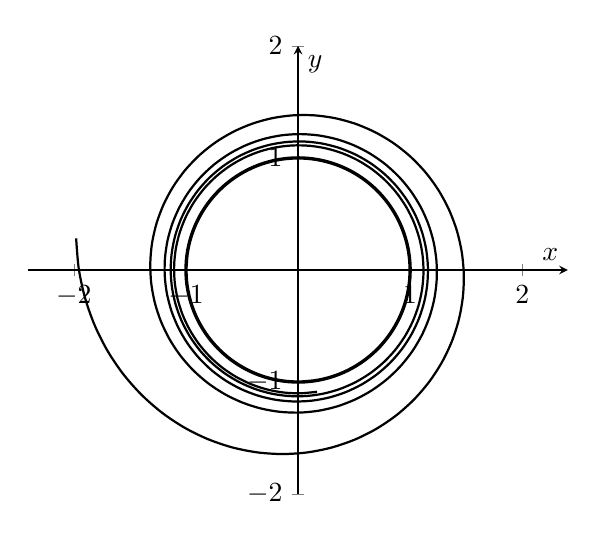
\begin{tikzpicture}[scale=1]
			\begin{axis}[
				axis lines = middle,
				xlabel = \(x\),
				ylabel = \(y\),
				xmin = -2,
				xmax = 2,
				ymax = 2,
				ymin = -2,
				axis equal,
				domain = 3:30,
				samples = 200,
				smooth,
				trig format plots=rad
				]
				\addplot[black, thick] ({(1+(3/x))*cos(x)}, {(1+(3/x))*sin(x)});
				\addplot[black, very thick] ({cos(x)}, {sin(x)});
			\end{axis}
		\end{tikzpicture} 
		\end{center}
		\[f(t)=
		\begin{cases}
			\left(\left(1+\frac1t\right)\cdot\cos{t}, \left(1+\frac1t\right)\cdot\sin{t}\right)\text{ - спираль}\\
			(\cos t,\ \sin t)\text{ - окружность}
		\end{cases}
		\]
		Заметим, что $D(f)$ является связным, но не линейно связным множеством.
\end{example}
